\autsubsection{Thermal Drilling}{Lukas Christensen}\label{sec:temp_simulation}
Most drilling methods convert electrical energy to some other form like, for example, kinetic or electro magnetic energy. During this conversion some amount of energy will be lost as heat to the environment and therefore not contribute to the drilling process. With thermal drills, however, this is not an issue since it is the heat itself that is used for the penetration process. This means that thermal drills are highly efficient, even though more energy is needed to melt a given material than to, say, break up its structure mechanically. Additionally, they are very simple to design and implement, since all that is needed is basically a heating element and an enclosure. It is even possible to use radioisotope thermal generators for the heating source, eliminating the need for any energy conversion in the drilling process.\\

\noindent
The calculations presented in section \ref{sec:IceTemperatureProfile} provide an initial estimate on the amount of thermal energy that is needed to penetrate the Europan ice sheet. Based on this, it would seem that melting through the ice can be achieved within realistic mission durations, however, more detailed calculations that take thermal loss in to account are needed before it is possible to conclusively choose a drilling method and optimize the design of the mission. \\

\noindent
A simulation has therefore been developed to accommodate this issue, however, it should be noted that a number of assumptions have been made in order to simplify the calculations somewhat. These include:
\begin{itemize}
	\item The ice sheet is homogeneous.
	\item The pressure variation throughout the ice has a negligible impact on the thermal characteristics.
	\item The bore hole closes and causes pressure build up to Earth atmospheric levels sufficiently fast that sublimation can be disregarded.
	\item The ice consists of pure water with no contents of salt or other pollutants.
\end{itemize}
The first assumption is probably not very realistic, but cracks in the ice and similar inhomogeneities will disrupt the conductive flow of heat thus result in a lower amount of heat transfer compared to the simulation results. This means that while the result of the simulation might not be completely realistic, it will represent a worst case scenario since less energy will likely be lost to the ice in reality. \\

\noindent
The second assumption should not result in significant deviations from reality as the melting point of water as well as the latent heat of fusion does not change significantly in the range of 1 to 100 atmospheres, which is the expected pressure range bearing in mind the third assumption. On the phase diagram presented in Figure \ref{fig:waterPhase} this is shown quite clearly with the boundary line between the solid and liquid state being near vertical at 273 K in the range of 1 kPa to 10 MPa.\\

\begin{figure}[ht]
	\centering
	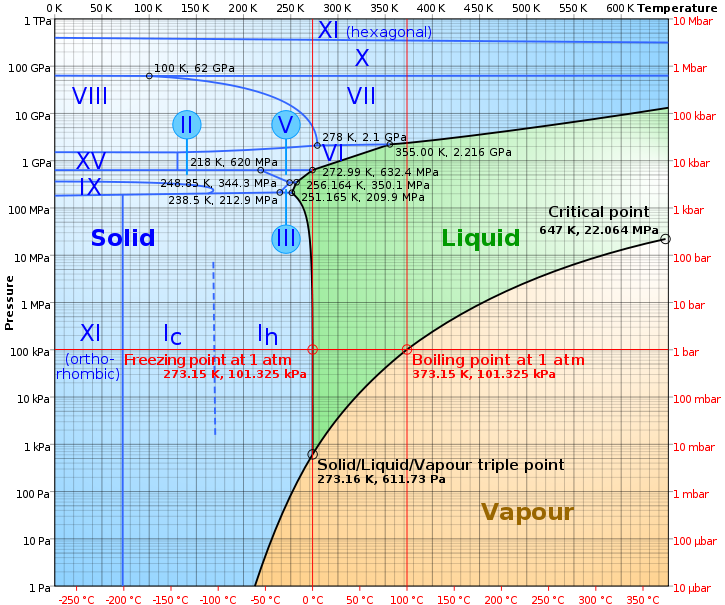
\includegraphics[width=8cm]{figures/LAMC/waterPhase}
	\caption{Phase diagram of water. Source: \url{http://math.ucr.edu/home/baez/chemical/725px-Phase_diagram_of_water.svg.png}}
	\label{fig:waterPhase}
\end{figure}

\noindent
The third assumption is probably fairly realistic considering that a relatively narrow penetrator ($\approx$ 20 cm diameter) is being considered. Naturally, at the beginning of the drilling process the ice will have to sublimate as the pressure is very close to vacuum, however, these sublimated ice particles will most likely adhere to the inner surface of the bore hole and make it narrower and narrower. After a while the bore hole will then close completely and pressure will star to build until sublimation is replaced by melting. How quickly this happens it quite critical considering that the sublimation energy is about 7 times\cite{website:engineeringToolbox} that of the melting energy. Experiments are needed to determine this exactly, but for now the simulation should still provide a decent estimate of the penetration time.\\

\noindent
The fourth assumption is most certainly not realistic and it will in all likelihood have a great deal of impact on the result, however, the implications of it will be discussed further in a separate section.

\subsubsection{Theory}
In order to evaluate the temperature evolution of a continuous fluid a good starting point is the equation of conservation of energy. For an incompressible fluid with no internal forces this is given by
\begin{equation}
\rho C \left( \mathbf{v} \cdot \nabla T + \frac{\partial T}{\partial t} \right) = \nabla (K \nabla T) + q 
\end{equation} 
Where $\rho$ is the density, $C$ is the heat capacity, $\mathbf{v}$ is the velocity of the fluid, $T$ is the temperature, $K$ is the thermal conductivity, and $q$ is added heat\cite{article:barr2014a}. Assuming no convection and a near constant thermal conductivity this reduces to
\begin{equation}
\label{eq:thermal1}
\frac{\partial T}{\partial t} = \frac{1}{\rho C}\left( K \nabla^2 T + q \right)
\end{equation}
For the case of a penetrator melting through the ice this equation becomes exceedingly difficult to solve analytically as the ice changes state during the melting and the heat source moves as a function of this. For this reason, it is advantageous to discretize the equation in order to facility computer simulations, which results in\\
\begin{equation} \label{eq:thermal2}
T_{k+1} \approx T_{k} + \frac{\partial T_{k}}{\partial t}\Delta t = T_{k} + \frac{\Delta t}{\rho_k C_k}\left( K_k \nabla^2 T_{k} + q_{k} \right)
\end{equation}
With $\Delta t$ being a small time step and $k$ being the current iteration number. Note that all the quantities in this equation, except $\Delta t$, need not be constant all over, but can vary spatially. Of course, ideally $K_k$ should only exhibit small variations in order to satisfy the earlier approximation. This is not strictly true at the interface between ice and water as there will be a discontinuous jump from $\SI{0.57}{\frac{W}{m K}}$ in the water to $\SI{2.22}{\frac{W}{m K}}$\cite{website:engineeringToolbox} in the ice, but the approximation should still be able to provide decent results.\\

\noindent
Once a volume $V$ of ice reaches its melting temperature, the amount of heat that is needed to convert it into water is equal to
\begin{equation}
Q_{melt} = \rho V L_{fus}
\end{equation}
Where $L_{fus} = \SI{333.5}{\frac{kJ}{kg}}$ is the latent heat of fusion of water\cite{article:biele2011a}.

\subsubsection{Implementation}
The actual simulation program have been implemented using Matlab as it easily accommodates scientific calculations on large matrices. The actual simulation algorithm is run on a 51x60x60 temperature matrix with each voxel representing a volume of 0.5x0.1x0.1 $\SI{}{m^3}$, totaling in a 25.5x6x6 $\SI{}{m^3}$ section of the ice sheet. As the heater melts through the ice, the grid moves with it thus eliminating the need for simulating the entire ice sheet at all times. The processing performed on the volume section is outlined in figure \ref{fig:iceSimFlow}.\\

 \begin{figure}[ht]
 	\centering
 	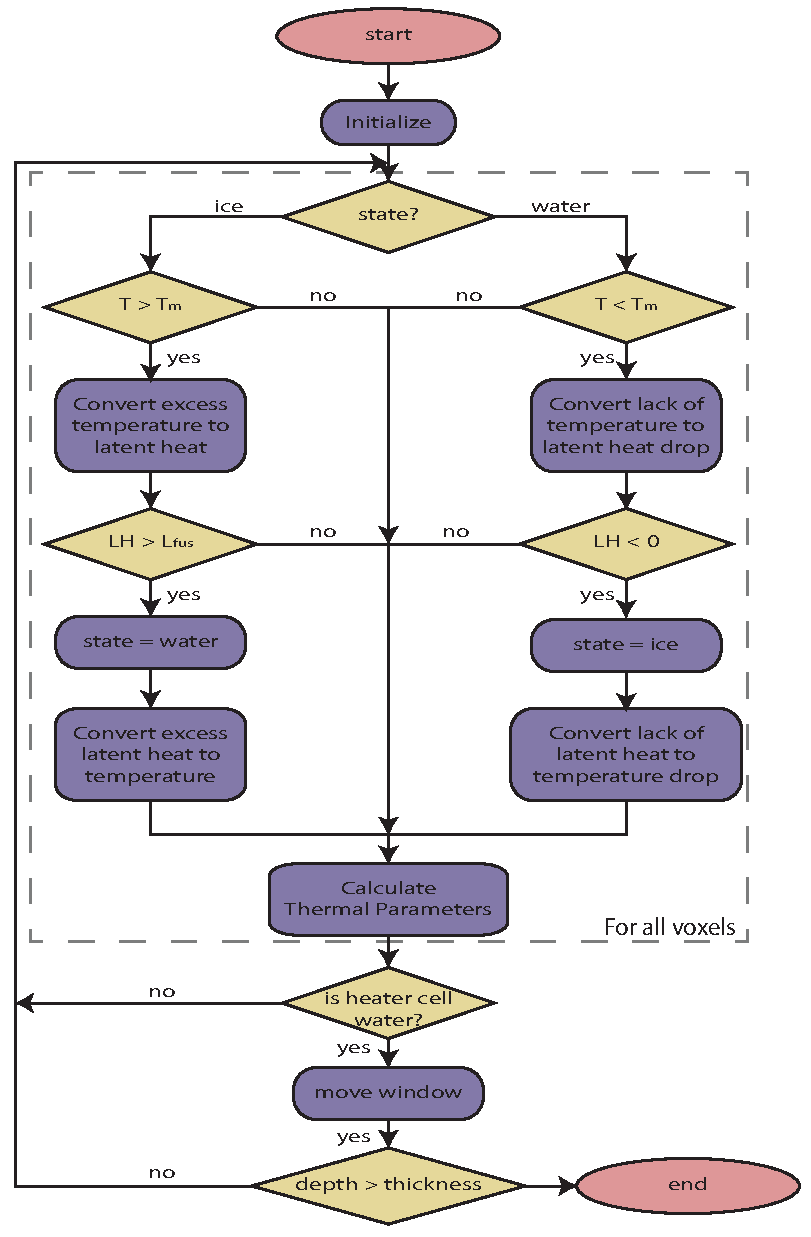
\includegraphics[width=.55\textwidth]{figures/LAMC/iceSimFlowchart.pdf}
 	\caption{Flowchart of the ice melting simulation.}
 	\label{fig:iceSimFlow}
 \end{figure}
 
\noindent
First, the change in temperature is calculated according to equation \ref{eq:thermal2} with the Laplacian being calculated using the Matlab command \texttt{del2()}. It is noteworthy that \texttt{del2()} actually, for whatever reason, returns $\frac{\nabla^2}{6}$ when working with 3D-coordinates. This change is then added to the current temperature value.\\

\noindent
At this point, the simulation branches out depending on whether a given grid cell is made up of water or ice. If it is an ice voxel, a check is made to see if the current temperature is above the melting point of ice. If this is the case, the excess temperature is converted to latent heat and stored in a separate matrix. If the latent heat is now above $L_{fus}$, the voxel is converted to water and the excess heat is converted to a temperature change and added to the current voxel.\\

\noindent
For a water voxel, the temperature is checked to see if it is below the melting point of water. If true, the temperature deficiency is converted and subtracted from the latent heat. If the latent heat now drops below 0, the cell is converted to ice and the negative latent heat is subtracted from the temperature (after being converted, of course).\\

\noindent
With the temperature and the state of each voxels being determined, the thermal parameters of each cell is determined by interpolating between points in a dataset that includes heat capacity, thermal conductivity and density for water and ice for a range of different temperatures. The dataset has been put together by combining information acquired from \cite{website:engineeringToolbox}. It should be noted that this data only covers the temperature interval 183-366 K and linear extrapolation has been used for temperatures outside of this range.\\

\begin{figure}[ht]
	\centering
	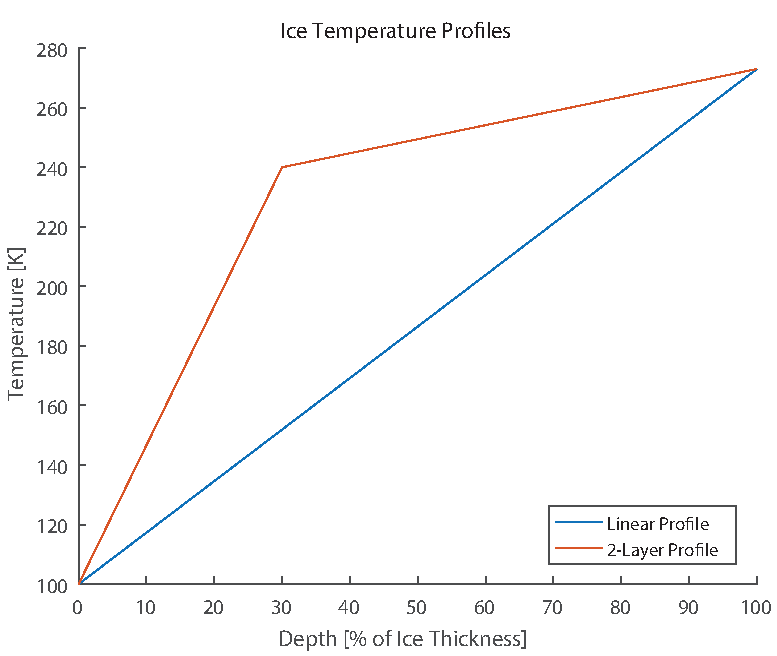
\includegraphics[width=.5\textwidth]{figures/LAMC/iceTempProfiles.pdf}
	\caption{The two temperature profiles used in the simulation: the linear based on calculations, and an approximated 2-layer profile based on the literature.}
	\label{fig:iceTempProfiles}
\end{figure}

\noindent
This basic flow is run for every voxel at every time step, until the heater makes it way through the ice sheet. The actual heater is implemented by injecting power in to a number of voxels that represent the extend of the heater. In the present configuration these consists of 4 cells located next to each other, however, not all the power is added to these. In order to accommodate the fact that the heating is distributed along the length of the penetrator, some of the power is injected in to the cells immediately above the heater. The exact amount is determined by a coupling coefficient, which is set to 99 \% in the used configuration meaning that 99 \% of the power is added to the heater cells and 1 \% percent is added to cells above. \\

\noindent
The amount of energy lost to heating the ice matrix and therefore not directly used to melt the ice below the penetrator is heavily influenced by this coupling coefficient. The used value was chosen as it seemed to match well with calculations that will be detailed in the validation section. To achieve a completely realistic result, real world experiments are needed to determine what the coupling coefficient should be set to.\\

\noindent
As soon as the heater voxels are converted to water, the entire simulation window together with the heater position is moved down by one increment of the vertical resolution. At the same time a depth variable is incremented by the same amount. Once this reaches the preset thickness of the ice sheet, the simulation is stopped. \\

 \begin{figure}[ht]
 	\centering
 	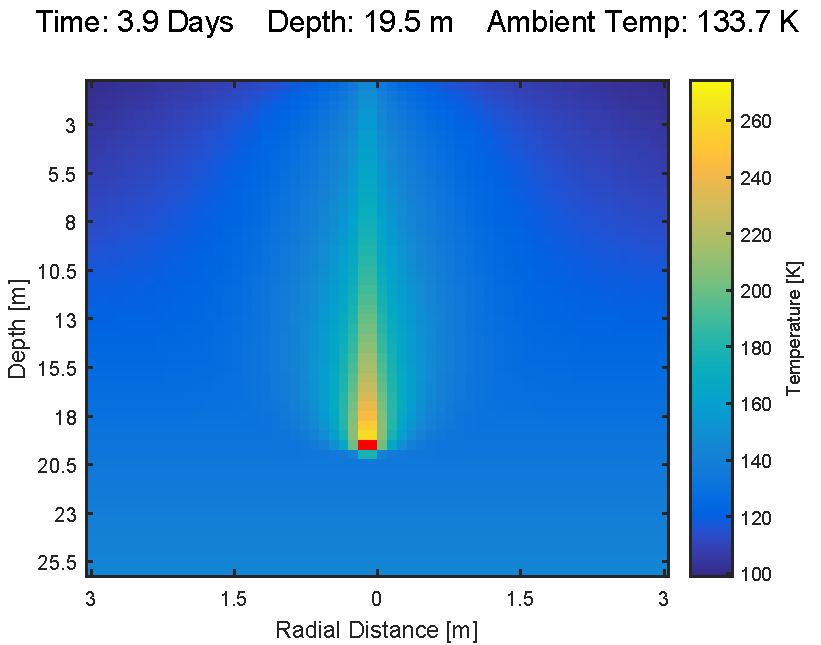
\includegraphics[width=0.5\textwidth]{figures/LAMC/snapshot.pdf}
 	\caption{Snapshot from the simulation program. This example is running with an ice thickness of 100 m, a linear temperature profile and a heater power of 2000 W. The red pixels indicate where the ice has melted and turned in to water. Videos of the running simulation are available at \url{https://www.youtube.com/watch?v=Rr-ucW9Br4A} and \url{https://www.youtube.com/watch?v=b72MfGw1ZE8}}
 	\label{fig:simSnapshot}
 \end{figure}

\noindent
The temperature that is loaded into the grid when the simulation is first initialized, as well as the temperature that is used to update the grid every time it moves, is calculated using a chosen temperature profile. Currently two differently profiles have been implemented namely the ones presented in sections \ref{sec:IceTemperatureProfile} and \ref{sec:IceTemperatureProfile2}: the linear one based on calculations, and an approximation of the two layer model with a thin cold layer followed by a thick warm layer. These profiles are plotted in figure \ref{fig:iceTempProfiles}.\\

\noindent 
A snapshot created during a run of the simulation is displayed in figure \ref{fig:simSnapshot}, clearly showing how a large part of the heating energy is being used to heat up the surrounding ice. The source code for the simulation is included in appendix \ref{app:iceSimCode}.


\subsubsection{Results}
Running the simulation with a constant heating power for a number of different ice thicknesses, it is clear that the penetration time is directly proportional to the ice thickness. This means that the simulation can be run with a thickness of just 100 m to reduce run times and still provide results that can be extrapolated to any arbitrary thickness. Furthermore, it is the power to cross-sectional area ratio that the determines the penetration time, meaning that only a few heating voxels are needed to get seemingly accurate results that can represent any given penetrator size. Running the simulation for a number of different heating values, but with a fixed heater size, results in figure \ref{fig:simResults}.

\begin{figure}[ht]
	\centering
	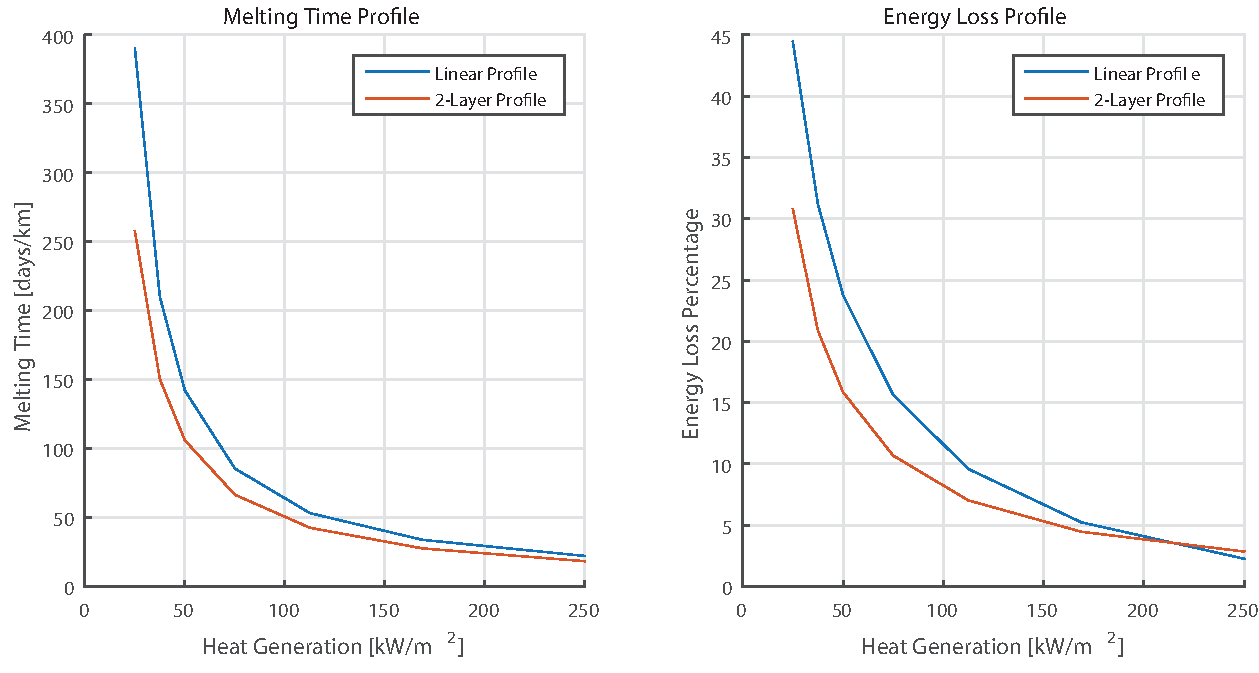
\includegraphics[width=.9\textwidth]{figures/LAMC/simResult.pdf}
	\caption{Result of the melting simulation. The left plot shows the penetration time per kilometer of ice for the two temperature profiles with varying heating densities, while the right shows the associated losses.}
	\label{fig:simResults}
\end{figure}

\noindent
The x-axis on the two graphs is equal to the total heater power divided by the cross-sectional area of the penetrator and loss percentage has been calculated as the ratio between the used energy and the energy needed to melt only the ice column the penetrator travels through. \\

\noindent
It can be seen that the both penetration time and loss percentage follows something similar to an exponentially decreasing curve. This means that the higher the power density the better, however, a point of diminishing returns is reached at around a heating density of $\SI{85}{\frac{kW}{m^2}}$. \\

\noindent
The working model of the penetrator has a 2 kW heater and a diameter of 20 cm meaning a heating density of $\SI{64}{\frac{kW}{m^2}}$ resulting in a loss of 19 \% and a penetration time of $\SI{111}{\frac{days}{km}}$ for the linear temperature profile, and 13 \% and $\SI{84}{\frac{days}{km}}$ for the 2-layer profile. So, for these penetrator dimensions it should be possible to design a mission with a realistic lifetime that can reach the bottom of the ice sheet. Granted, this requires that the ice has a modest thickness; with much more than 5 km of ice multiple years are needed for the penetration which is probably not realistic.\\

\noindent
If the ice sheet is found to be unreasonably thick, one option will be to reduce the diameter of the penetrator. Changing the design to a diameter of 15 cm instead results in penetration times of $\SI{42}{\frac{days}{km}}$ to $\SI{53}{\frac{days}{km}}$, depending on the temperature profile. This would enable a doubling of the ice thickness while maintaining the same mission duration. Of course, this would require a redesign of the mission, but the option is available. Alternatively, increasing the heater power by 80 \% would result in the same gain in power density. 

\subsubsection{Verification}
The simulation has provided results that show the mission to possible, however, these results need to be verified to make sure that the simulation reflects the real world.\\

\noindent
According to Biele et al. (2011)\cite{article:biele2011a}, the amount of power that is lost to heating up the ice around a heating element is equal to
\begin{equation}
P_{cond}=\frac{4 K (T_m-T) }{R\pi^2}(2\pi R)\times \int_{0}^{H}\int_{0}^{\infty}\frac{
e^{-\kappa u^2 s/v}
}{
u\left[J_0^2(R u) + Y_0^2(R u)\right]
}duds
\end{equation}
Where $T_m$ is the melting temperature, $T$ is the temperature of the ice, $R$ is the radius of the heater, $H$ is the length of the heater, $\kappa=\frac{K}{\rho C}$ is the heat diffusion coefficient, $v$ is the downward speed of the heater, and $J_0^2$ and $Y_0^2$ are the first two Bessel functions of zero'th order. The total power needed to move at a given speed is then equal to
\begin{equation}
P_{tot} = A\rho v(C(T_m-T) + L_{fus}) + P_{cond}
\end{equation} 
With $A=\pi R^2$ being the cross-sectional area of the heater. In the case of the penetrator, the velocity is not known, but the total power is. By numerically solving $P_{tot}$ equal to some given power, the velocity, and by extension $P_{cond}$ can be determined. Afterwards, the velocity can be integrated to find the penetration time, and the total loss can be calculated from $P_{cond}$. Performing this process for a number of different heater powers and the two temperature profiles results in figure \ref{fig:verificationResult}.

\begin{figure}[ht]
	\centering
	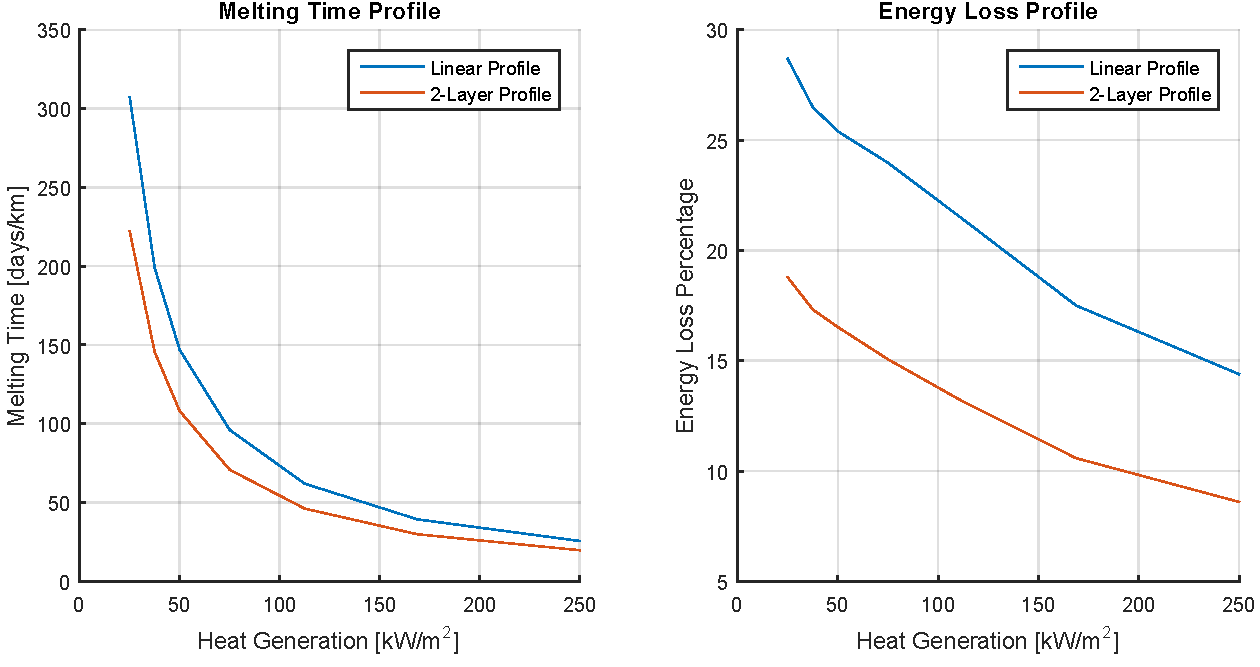
\includegraphics[width=.9\textwidth]{figures/LAMC/verificationResult.pdf}
	\caption{Result of solving the loss power equation for different heater densities. The left plot shows the penetration time per kilometer of ice. The right shows the calculated losses. Cross-section of $\SI{0.04}{m^2}$ was used together with a heater length of 0.15 m.}
	\label{fig:verificationResult}
\end{figure}

\noindent
By comparing this to figure \ref{fig:simResults}, it is clear that there are discrepancies between the simulated and the calculated losses: For low power densities the simulation overestimates the losses, and for the high densities the simulation results in much too low losses. Even so, there is a very good match in the penetration times, with a deviation below $\SI{8}{\frac{days}{km}}$ for most power densities and with an absolute maximum at the lowest heating density of  $\SI{80}{\frac{days}{km}}$. This indicates that the simulation does, indeed, provide realistic results. The reason that the penetration times can be similar, even though the losses are different, is probably that the difference in loss is largest at the high power densities where the penetration time is the shortest. This means that the errors have less time to accumulate resulting in lower overall differences.\\

\noindent
To generate these graphs a cross-sectional area of $\SI{0.04}{m^2}$ and a heater length of 0.15 m was used. The choice of the heater length is meant to reflect that most of the heating power will be situated in the front of the penetrator. Of course, this is not an entirely physically correct picture, since some power will distributed through the penetrator to keep the instruments at a pleasant temperature and to make sure that the top of the does not get stuck in refreezing ice. Additionally, the density, heat capacity and thermal conductivity are assumed to be constant throughout the ice, further simplifying the picture. However, seeing as the calculations and the simulations provide very similar results it is probably safe to assume that the results can be trusted to reflect the real world, at the very least as a first approximation.\\

\subsubsection{Salinity} \label{sec:iceSalinity}
As previously mentioned, the ice will certainly include some amount of salts and other pollutants, however the actual concentration and composition is still unknown. These pollutants will most definitely have an effect on the penetration time, but it is difficult to find numerical values for the thermal properties at different salinities and temperatures - especially for other salts than sodium chloride. However, \citet{book:thomas2009sea} states that for sea ice these parameters can be approximated by empirical formulae:\\

\noindent
For the thermal conductivity, the following relation holds
\begin{equation}
K_{si}=\frac{\rho_{si}}{\rho_i}\left(2.11 - 0.011 T + 0.09 \frac{T}{S} - \frac{\rho_{si}-\rho_i}{1000}\right)\SI{}{\frac{W}{m K}}
\end{equation}
Where $\rho_{si}$ is the density of sea ice (on average $\SI{910}{\frac{kg}{m^3}}$\cite{article:timco19961}), $\rho_i$ is the density of pure water ice ($\SI{927}{\frac{kg}{m^3}}$), $T$ is the temperature measured in $^\circ C$ and $S$ is the salinity in ppt.\\
Similarly, the heat capacity can be approximated as
\begin{equation}
C_{si} = \left(2.11 + 17.2 \frac{S}{T^2}\right)\SI{}{\frac{kJ}{kg K}}
\end{equation}
And finally, the latent heat of fusion is given by
\begin{equation}
L_{si}=\left(333.4-2.11T-0.114S+18.1\frac{S}{T}\right)\SI{}{\frac{kJ}{kg}}
\end{equation}

\noindent
Plotting these equations for varying temperatures and salinities results in figure \ref{fig:iceSalinity}.
\begin{figure}[ht]
	\centering
	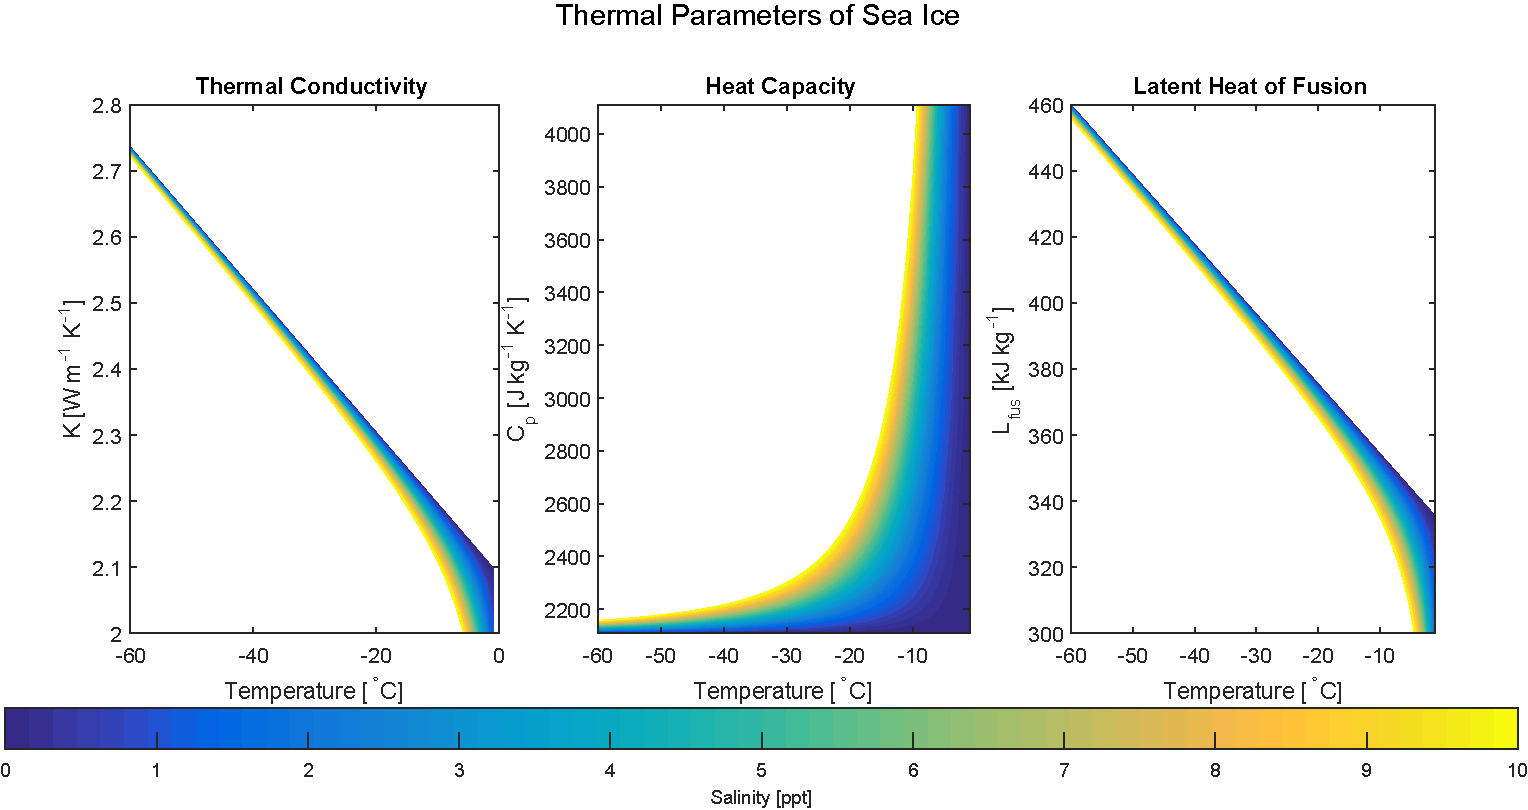
\includegraphics[width=.9\textwidth]{figures/LAMC/salinity}
	\caption{Thermal parameters of sea ice as a function of temperature and salinity.}
	\label{fig:iceSalinity}
\end{figure}
As can be seen, both the thermal conductivity and the latent heat of fusion decreases with increasing salinity, while the heat capacity increases. \\

\noindent
The increase of the heat capacity will result in more energy being needed to heat up the ice, which will work towards increasing the penetration time. On the other hand, the decreasing heat of fusion and thermal conductivity will mean that less energy is needed for the melting process and there will be an overall lower loss as less heat is conducted away from the penetrator.\\

\noindent
Seeing as the latent heat accounts for some 65-80\% of the ideal amount of energy needed to melt through the ice, it would seem that the decrease in the latent heat of fusion alone would outweigh the increase in heat capacity. Combining this with the decrease in thermal conductivity as well strongly indicates that salinity will actually work in favor of the mission and decrease the penetration time. Besides these effects the addition of salt also lowers the melting point of ice, further indicating salinity to be advantageous. Of course, these empirical formulas are designed to work with sea ice containing mainly NaCl while the composition of the Europan pollutants is unknown. It seems likely, however, that other salts will have similar effects. 

\subsubsection{Conclusion}
A simulation has been developed that is able to estimate the decent time of a ice melting probe, given its cross-section, heating power and the temperature profile of the ice. The calculations are based on the characteristics of pure water ice, but the implications of pollutants have been discussed and shown, in all likelihood, to reduce the total penetration time. The simulation has also been shown to be in good compliance with results calculated using approximate formulas that are often used in the field of thermal ice probes, thus indicating that the results are realistic. \\

\noindent
The results of the simulation point toward a penetration time of approximately $\SI{100}{\frac{days}{km}}$ for a penetrator with a diameter of 20 cm and a 2000 W heater. This means that melting is a feasible method for getting through the Europan ice sheet within realistic time frames and using reasonable designs. This, combined with the high degree of simplicity associated with heating compared to other drilling methods, means that melting is an excellent candidate for the technology to be used for ice penetration. As such, melting is the method of choice for this mission.

\subsubsection{Future Work}
The heating simulation that has been developed strongly indicates that total ice sheet penetration can be achieved within realistic time frames, however, there are a number of ways the simulation can be expanded and made to reflect reality closer.\\

\noindent
Currently, the simulation only operates on a small subsection of the ice at any given time. This means that some accuracy is lost as the cold wave moving from the top of the bore hole towards the penetrator might not be properly realized. A similar issue arises when the heat wave expanding radially outwards from the heater reaches the edges of the window. Additionally, the resolution is fairly coarse meaning that detailed information about the temperature gradient close to the penetrator is not attainable.\\
These issues could be alleviated by using a larger simulation window and better resolution at the expense of computation time. Implementing a adaptive grid with a spatially varying resolution would be a good way to reduce the computation time considerably and at the same time gain a larger window and a finer resolution where it is needed. It would also be advantageous to use cylindrical coordinates instead of Cartesian given the symmetry of the situation.\\

\noindent
Using the empirical models for sea ice, the simulation could be extended to include the effect of salinity in order to investigate whether the penetration time is indeed lowered as simple analysis suggest. The effects of other compounds than sodium chloride should also be investigated, however, this will likely require extensive experimental work as many different compositions might exist on Europa.\\

\noindent
At the moment, the integration is done in a fairly naive manner by simply adding the calculated time derivative multiplied by the time step to the current temperature. While this works fine for short time steps, it quickly breaks down causing numerical instabilities as the time step is increased. By implementing more sophisticated integration algorithms the time step could be increased, drastically reducing run times and increasing the accuracy of the simulation simultaneously.\\

\noindent
The simulation works on a grid with a fixed element size. The result of this is that the volume changes that are associated with the phase change of water are not taken into account. While this should not have a great effect on the ice melting itself, it should be evaluated as it affects how the bore hole refreezes. It will also result in a change in pressure, something that the simulation is currently unable to deal with. These effects should also be accounted for, for the simulation to be as accurate as possible.\\

\noindent
Finally, there is the issue of the coupling coefficient. This semi-physical parameter has an enormous influence on the amount of energy loss and by extension the penetration time. As mentioned, this was more or less arbitrarily chosen to best match the result of the analytical expressions for the power loss as well as possible. However, this is not exactly ideal as it is hard to determine how well this reflects reality. Experiments should be conducted to determine how this coefficient varies as the configuration of the heater is changed.     


